\documentclass[a4paper, 12pt]{article}

\usepackage{listings}
\usepackage{color}

\definecolor{dkgreen}{rgb}{0,0.6,0}
\definecolor{gray}{rgb}{0.5,0.5,0.5}
\definecolor{mauve}{rgb}{0.58,0,0.82}

\lstset{frame=tb,
	language=C,
	aboveskip=3mm,
	belowskip=3mm,
	showstringspaces=false,
	columns=flexible,
	basicstyle={\small\ttfamily},
	numbers=none,
	numberstyle=\tiny\color{gray},
	keywordstyle=\color{blue},
	commentstyle=\color{dkgreen},
	stringstyle=\color{mauve},
	breaklines=true,
	breakatwhitespace=true,
	tabsize=3
}

\usepackage[english]{babel}
\usepackage{microtype}
\usepackage{graphicx}
\usepackage{amsmath}
\usepackage{index}

\makeindex

\begin{document}
	\title{Tutorat microprocesseur}
	\author{Corentin , Florian DERLIC, Miaoqi WANG, Maxence NEUS}
	\maketitle
	
	\newpage
	\tableofcontents
	\newpage
	
	\section{Introducion}
		Nous avons à réaliser un radar de contrôle routier.
		Le radar doit pouvoir réaliser les fonctions suivantes :
		\begin{enumerate}
			\item Mesurer la vitesse d'un véhicule qui entre dans sa zone d'action
			\item Permettre de changer la vitesse maximale authorisée à l'aide d'un clavier
			\item Si la vitesse mesurée est supérieure à la vitesse maximale, activer le flash et envoyer la vitesse mesurée sur l'imprimante série
		\end{enumerate}
	\newpage
	\section{Architecture Matérielle}
		\subsection{Matériel}
		Nous avons à notre dispositon les éléments suivants :
		\begin{itemize}
			\item Un télémetre qui fournit un signal analogique proportionnel à la distance entre le radar et la voiture
			qui donne une valeur entre 0V pour une distance de 0m et 5v pour une distance de 100m
			\item Un détecteur de présence qui passe de l'état 0 à l'état 1 lorsqu'une voiture entre dans le champ de mesure du télémetre
			\item Un flash que l'on peut déclancher directement sur un pin digital
			\item Une imprimante série pour imprimer les vitesses mesurées
			\item Les composants standards
		\end{itemize}	
		\subsection{Mise en place de l'architecture}
		\begin{figure}[h]
		\centering
		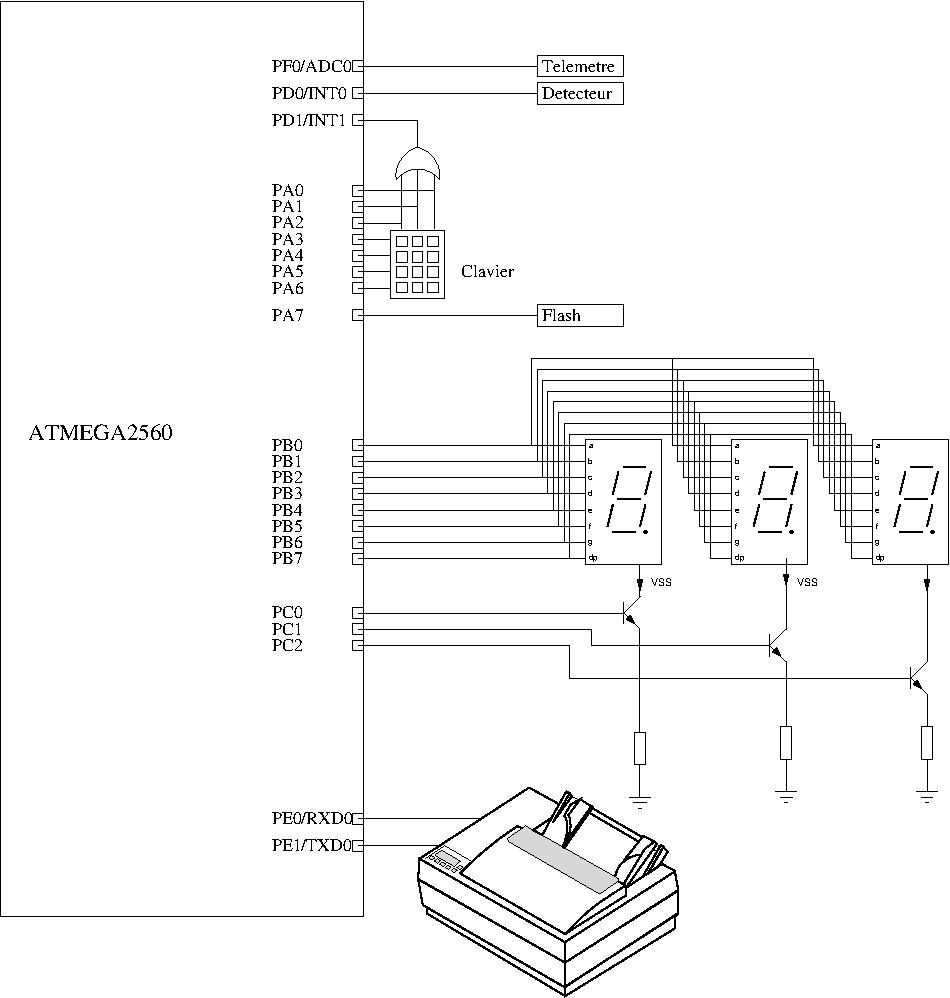
\includegraphics[width = 9cm]{schema.jpg}
		\caption{schema de cablage}
		\end{figure}
		\newpage
		\subsubsection{Interface utilisateur}
		Pour réaliser la fonction 2, nous avons besoin de permettre à l'utilisateur de rentrer une nouvelle valeur pour la vitesse maximale authorisée. Pour ce faire, nous avons incorporer un clavier 12 touches (0-9, Valider, Annuler) et 3 afficheurs 7 segments multiplexés pour afficher la valeur entrée à l'utilisateur.\\
		Le clavier est branché sur les pins PA[0:6] avec une porte OU qui permettra par la broche PD1/INT1 de travailler par interruption pour la lecture du clavier.\\
		Pour ce qui est des afficheurs 7 segments, ils sont reliés au port B pour la valeur à afficher et multiplexé par les pins PC[0:2] qui font la conection des bases des afficheurs à la masse via des transistors et des résistances de tirage.
		\subsubsection{Appareils de mesure}
		Comme le Télémetre nous fournis une valeur analogique, nous avons choisis de le relier à la broche PF0/ADC0 pour pouvoir réaliser une conversion dessus.\\
		Nous avons choisis d'utiliser le détecteur de présence par intéruption, nous le relions donc à la broche PD0/INT0.\\
		\subsubsection{Sorties utilisateur}
		Pour le flash, nous l'avons relié à la dernière broche inutilisée du port A, PA7, nous supposons qu'un appareil photo déclanchable par un front montant est relié à la même broche pour pouvoir prendre une photo de l'automobiliste qui est en exces de vitesse.\\
		L'impimante série est reliée à l'interface USART0 (PE0/RXD0;PE1/TXD1), L'imprimante fonctionne à 1200 bauds, 8bits de message, 1 bit stop et pas de parité, son initialisation sera développée dans la section 3.\\
	\newpage
	\section{Architecture Code}
		\subsection{Initialisation}
		\begin{lstlisting}
			//ADC (convertion ADC0, single convertion)
			ADMUX = 0b0010 0000
			ADCSRA = 0b1000 1111
			ADCSRB = 0x00
		\end{lstlisting}
		
		\begin{lstlisting}
			//Watchdog (interruptions toute les 0.5s)
			WDTCSR = 0x10 // enable change
			WDTCSR = 0b0101 0101
		\end{lstlisting}

		\begin{lstlisting}
			//printer (envoi uniquement, pas de verification, conforme au CDCF)
			UBRR (f = 16MHz) = 832
			UBRRH0 = 0x03
			UBRRL0 = 0x40
			
			UCSR0A = 0x00
			UCSR0B = 0b0000 1000
			UCSR0C = 0b0000 0110			
		\end{lstlisting}	
	
		\begin{lstlisting}
			//Clavier et afficheurs
			DDRA = 0b0001 1111
			DDRB = 0x0111 1111
			DDRC = 0b0000 0111
		\end{lstlisting}
		
		\begin{lstlisting}
			//vecteurs d'interuption
			.org 0x0002
				JMP IRQ_detecteur
			.org 0x0004
				JMP IRQ_clavier
			.org 0x0018
				JMP IRQ_Watchdog
			.org 0x003A
				JMP IRQ_convertion
		\end{lstlisting}
\end{document}